%%%%%%%%%%%%%%%
%
% $Autor: Wings $
% $Datum: 2020-01-29 07:55:27Z $
% $Pfad: Nano33BLESense.tex $
% $Version: 1785 $
%
%
%%%%%%%%%%%%%%%


\chapter{Arduino Nano 33 BLE Sense}

Arduino ist eine Open-Source-Elektronikplattform, die auf flexibler und benutzerfreundlicher Hardware sowie Software basiert. Sie bietet Mikrocontroller- und Mikroprozessor-Boards zur Entwicklung digitaler und analoger Geräte.

Der Mikrocontroller - oft als "Mini-Computer" des Arduino-Boards bezeichnet - benötigt normalerweise verschiedene elektronische Bauteile wie Dioden, Widerstände, Kondensatoren und Transistoren zur Spannungs- und Stromregulierung. Das Arduino-Team hat jedoch eine benutzerfreundliche Umgebung geschaffen, die diese elektronischen Komplexitäten überflüssig macht:

\begin{itemize}
	\item Einfache Stromversorgung nach Spannungsvorgabe
	\item Programmierung in wenigen Sekunden
	\item Automatische Hardware-Steuerung
	\item Keine zusätzlichen elektronischen Komponenten erforderlich
\end{itemize}

Durch Fortschritte in der Halbleiter- und Elektronikindustrie werden Steuerungsprobleme heute zunehmend mit diesen kompakten Mikrocontrollern gelöst, anstatt mit mechanischen oder elektrischen Schaltern.\cite{Arduino:2025}


\section{Arduino Nano 33 BLE Sense}

Die Arduino Nano-Familie umfasst kompakte Boards mit umfangreichen Funktionen – vom preisgünstigen Einsteigermodell Nano bis hin zum funktionsreichen Nano BLE Sense/Nano RP2040 Connect mit Bluetooth-/Wi-Fi-Modulen. Diese Boards verfügen über integrierte Sensoren für Temperatur, Luftfeuchtigkeit, Druck, Gestenerkennung, Mikrofon und mehr. Sie unterstützen zudem MicroPython und Machine Learning \cite{Raj:2019}.

Das Arduino Nano 33 BLE Sense ist ein kompaktes Board der Nano-Familie mit:
\begin{itemize}
	\item Bluetooth Low Energy (BLE 5.0) über das NINA-B306-Modul
	\item Leistungsstarkem Nordic nRF52480-Prozessor (Cortex M4F)
	\item Umfangreicher Sensorik:
	\begin{itemize}
		\item 9-Achsen-IMU (Beschleunigungssensor, Gyroskop, Magnetometer)
		\item Umwelt-Sensoren (Temperatur, Luftfeuchtigkeit, Druck)
		\item Optische Sensoren (RGB-Licht, Gesten, Näherung)
		\item Digitales Mikrofon
	\end{itemize}
	\item Energieeffizientem Design im Nano-Format (45x18mm)
\end{itemize}

\subsection*{Namenskonvention}
Die Bezeichnung gibt Aufschluss über die Funktionen:
\begin{itemize}
	\item \textbf{Nano}: Kompakte Bauform (45x18mm)
	\item \textbf{33}: Betriebsspannung 3.3V
	\item \textbf{BLE}: Bluetooth Low Energy 5.0
	\item \textbf{Sense}: Integrierte Sensor-Suite
\end{itemize}

\subsection*{Erweiterungsmöglichkeiten}
Für erweiterte Anwendungen wie:
\begin{itemize}
	\item RGB-Farberkennung
	\item Objekterkennung
	\item Gestensteuerung
\end{itemize}
lässt sich das Board mit dem Arducam OV2640-Kameramodul kombinieren. Diese Kombination eignet sich ideal für Machine-Learning- und KI-Anwendungen – die notwendigen Bibliotheken stehen in der Arduino IDE zur Verfügung.

Folgende Abbildung zeigt den Arduino Nano 33 BLE Sense. \ref{ArduinoNano33}

\begin{center}
\begin{tikzpicture}
  \ArduinoNanoBLESenseRev
\end{tikzpicture}  
    \captionof{figure}{Arduino Nano 33 BLE Sense Rev. 2, see \href{https://store.arduino.cc/arduino-nano-33-ble-sense}{Arduino Store}} 
    \label{ArduinoNano33}
\end{center}

\subsection*{Technische Spezifikationen des Arduino Nano 33 BLE Sense}

Das kompakte und zuverlässige BLE-Board basiert auf dem NINA-B306-Modul für Bluetooth Low Energy (BLE 5.0). Dieses Modul enthält den leistungsstarken Nordic nRF52480-Prozessor mit Cortex-M4F-CPU und ist vollständig kompatibel mit der Arduino IDE (online und offline). \cite{Arduino:2025}

\subsection*{Integrierte Sensoren und Komponenten}

\begin{itemize}
	\item \textbf{Funkmodul}:
	\begin{itemize}
		\item NINA-B306-Modul für Bluetooth 5.0 LE
		\item Reichweite bis zu 100m (freies Feld)
		\item Datenrate bis zu 2Mbit/s
	\end{itemize}
	
	\item \textbf{APDS-9960 Sensor}:
	\begin{itemize}
		\item Integrierter RGB-, Gesten- und Näherungssensor
		\item Messbereich: 0-255 für RGB-Werte
		\item Gestenerkennung (Links/Rechts/Oben/Unten)
	\end{itemize}
	
	\item \textbf{LSM9DS1 IMU}:
	\begin{itemize}
		\item 9-Achsen-Inertialsensor (Beschleunigung, Gyroskop, Magnetometer)
		\item Beschleunigungsbereich: ±2/±4/±8/±16 g
		\item Gyroskop-Bereich: ±245/±500/±2000 °/s
	\end{itemize}
	
	\item \textbf{LPS22HB Drucksensor}:
	\begin{itemize}
		\item Messbereich: 260-1260 hPa
		\item Temperaturbereich: -40°C bis +85°C
	\end{itemize}
	
	\item \textbf{HTS221 Feuchtesensor}:
	\begin{itemize}
		\item Relative Luftfeuchtigkeit: 0-100% RH
		\item Genauigkeit: ±3.5\% RH
	\end{itemize}
	
	\item \textbf{MP34DT05 Mikrofon}:
	\begin{itemize}
		\item Digitales MEMS-Mikrofon
		\item Frequenzbereich: 100Hz-16kHz
		\item Signal-Rausch-Verhältnis: 64dB
	\end{itemize}
	
\end{itemize}


\section{Unterschied zwischen dem Arduino Nano 33 BLE Sense Rev1, dem Arduino Nano 33 BLE Sense Rev2 und dem Arduino Nano 33 BLE Sense Lite}

\subsection{Worin unterscheiden sich Rev1 und Rev2?}

Die Unterschiede zwischen dem Arduino Nano 33 BLE Sense und der Rev2-Version betreffen folgende Komponenten: IMU, Temperatur- und Feuchtesensor, Mikrofon, Krypto-Chip und Spannungswandler. In der zweiten Revision wurde:

\begin{itemize}
	\item Die LSM9DS1-IMU durch zwei separate Module ersetzt:
	\begin{itemize}
		\item BMI270 (Beschleunigungs- und Drehratensensor)
		\item BMM150 (Magnetometer)
	\end{itemize}
	
	\item Der HTS221-Feuchtesensor durch den präziseren HS3003
	
	\item Das Mikrofon MP34DT05 durch den MP34DT06JTR (bei gleichen Spezifikationen)
	
	\item Der Spannungswandler MPM3610 durch den MP2322
	
	\item Der Krypto-Chip vollständig entfernt
	
\end{itemize}

\subsection*{Zusammenfassung der Änderungen}

\begin{itemize}
	\item \textbf{IMU}: Ersatz des 9-Achsen-LSM9DS1 durch BMI270 (6-Achsen) + BMM150 (3-Achsen)
	\item \textbf{Umweltsensor}: HTS221 zu HS3003 (höhere Genauigkeit)
	\item \textbf{Mikrofon}: MP34DT05 zu MP34DT06JTR (funktional identisch)
\end{itemize}

\subsection*{Verbesserte Nutzerfreundlichkeit}

\begin{itemize}
	\item \textbf{Stromversorgung}: MPM3610 zu MP2322 (effizienter)
	\item \textbf{VUSB-Lötpad}: Neu auf der Oberseite der Platine
	\item \textbf{Testpunkte}: Für USB, SWDIO und SWCLK hinzugefügt
\end{itemize}

\begin{center}
	\begin{tikzpicture}
		\ArduinoNanoBLESenseOne
	\end{tikzpicture}
	\captionof{figure}{Arduino Nano 33 BLE Sense Rev. 1}
	\label{ArduinoNano33One}
\end{center}

\subsection*{Anpassungen in Sketches}

Für bestehende Sketches müssen folgende Bibliotheken angepasst werden:

\begin{itemize}
	\item \textbf{IMU}: LSM9DS1 zu ArduinobBMI270bBMM150
	\item \textbf{Umweltsensor}: HTS221 zu Arduino HS300x
\end{itemize}

\bigskip

Rev 1 TensorFlow Lite Bibliothek: \
\HREF{https://downloads.arduino.cc/libraries/github.com/bcmi-labs/Arduino_TensorFlowLite-1.15.0-ALPHA.zip 3}{TensorFlow Lite lib}


\subsection{Arduino Nano 33 BLE Sense Lite}

Das Tiny Machine Learning Kit enthält ausschließlich die Arduino Nano 33 BLE Sense Lite Version.

\subsubsection{Unterschiede zur Rev1}
Die Lite-Variante unterscheidet sich nur minimal vom Arduino Nano 33 BLE Sense Rev1:
\begin{itemize}
	\item \textbf{Fehlender Sensor}: Der HTS221 (Feuchtigkeit und Temperatur) wurde entfernt
	\item \textbf{Alternative Temperaturmessung}: Kann über den verbleibenden LPS22HB Drucksensor erfolgen
	\item \textbf{Einschränkung}: Keine Messung der relativen Luftfeuchtigkeit möglich
\end{itemize}

\subsubsection{Technische Hintergründe}
\begin{itemize}
	\item \textbf{Entscheidungsgrund}: Lieferkettenprobleme bei der Beschaffung des HTS221 Sensors
	\item \textbf{Kompensation}: Externe Feuchtesensoren können über I²C angeschlossen werden
	\item \textbf{Kostenvorteil}: Geringerer Stückpreis durch reduzierten Sensorumfang
\end{itemize}
\cite{Paradise:2025}
\begin{center}
	\begin{tikzpicture}
		\ArduinoNanoBLESenseLLite
	\end{tikzpicture}
	\captionof{figure}[Arduino Nano 33 BLE Sense Lite]{Arduino Nano 33 BLE Sense Lite; Das leere schwarze Quadrat markiert die Position des fehlenden HTS221 Sensors}
	\label{ArduinoNano33OneLite}
\end{center}


\section{Beschreibung der On-Board Sensoren}

Der Arduino Nano 33 BLE Sense verfügt über eine Reihe integrierter Sensoren zur Messung analoger und digitaler Umgebungswerte. Mit seinen kompakten Abmessungen von nur 45mm × 18mm eignet er sich ideal für IoT- und KI-Anwendungen, bei denen Platzbeschränkungen eine Rolle spielen. Das Board hat einen geringen Stromverbrauch und arbeitet mit 3,3 V, wodurch es monatelang mit kleinen Batterien betrieben werden kann. Dank der integrierten Sensoren, des niedrigen Energieverbrauchs und der kompakten Bauweise kann dieses Nano-Board vielseitig eingesetzt werden. Der Arduino Nano 33 BLE Sense ist ein völlig neues Board in bekanntem Formfaktor. Detaillierte Informationen zu den Komponenten und Datenblätter der Sensoren finden Sie unter \cite{ArduinoWeb:2025}.

Die Sensoren im Überblick:

\begin{itemize}
	\item Der APDS-9960 ist ein digitaler Sensor für Näherung, Umgebungslicht, RGB und Gesten. Er misst Entfernung, Licht, Farbe und Gesten in Boardnähe.
	\item Der LSM9DS1 ist ein 9-Achsen-\ac{imu} (Beschleunigungsmesser, Gyroskop und Magnetometer), ideal für Wearables.
	\item Der LPS22HB ist ein barometrischer Drucksensor zur Messung des Umgebungsdrucks, nützlich für einfache Wetterstationen.
	\item Der HTS221 misst relative Luftfeuchtigkeit und Temperatur für präzise Umgebungsdaten.
	\item Der MP34DT05 ist ein digitales Mikrofon zur Echtzeiterfassung und Analyse von Geräuschen.
	\item Der USB-Port ermöglicht die Verbindung mit einem Computer.
	\item Das Board hat drei LEDs: eine programmierbare RGB-LED, eine orange Status-LED und eine Power-LED.
\end{itemize}

Abbildung \ref{ArduinoNano33BLESenseArchitecture} zeigt die Anordnung der Sensoren auf dem Board sowie den leistungsstarken nRF52840-Prozessor von Nordic Semiconductors, einen 32-bit ARM\textsuperscript{\textregistered} Cortex\textsuperscript{\texttrademark}-M4 mit 64 MHz Taktfrequenz.

\begin{center}
	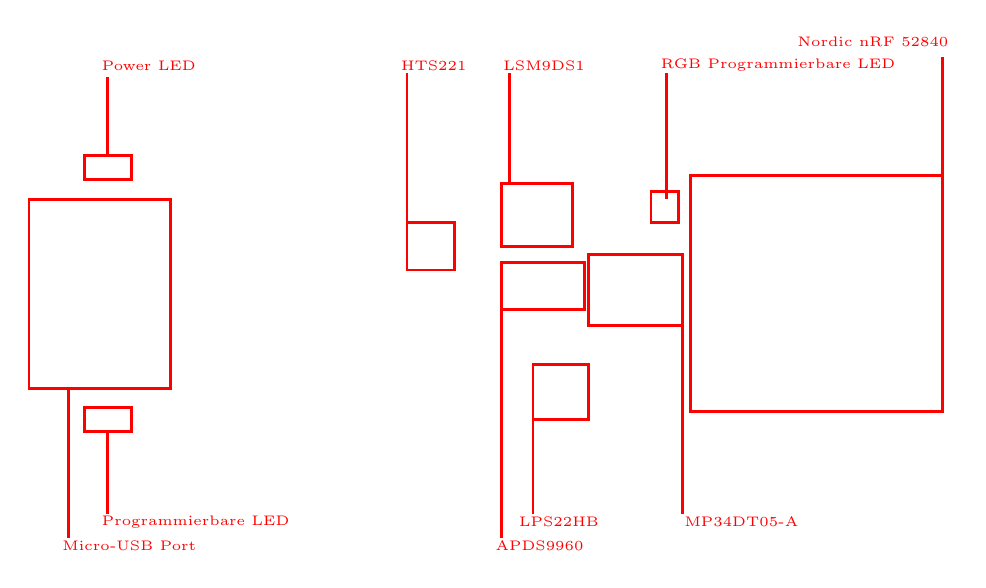
\begin{tikzpicture}
		\ArduinoNanoBLESenseOne
		
		\node[right](LEDPower) at (0.5,5.4){\textcolor{red}{\tiny Power LED}};
		\draw[line width=1pt,red]  (0.7,5.25) -- (0.7,4.25);
		\draw[line width=1pt,red] (0.4,4.25) -- (1.0, 4.25) -- (1.0,3.95) -- (0.4,3.95) -- cycle;
		
		\node[right](HTS) at (4.3,5.4){\textcolor{red}{\tiny HTS221}};
		\draw[line width=1pt,red]  (4.5,3.4) -- (4.5,5.3);
		\draw[line width=1pt,red] (4.5,3.4) -- (5.1, 3.4) -- (5.1,2.8) -- (4.5,2.8) -- cycle;
		
		\node[right](LSM9DS1) at (5.6,5.4){\textcolor{red}{\tiny LSM9DS1}};
		\draw[line width=1pt,red]  (5.8,3.9) -- (5.8,5.3);
		\draw[line width=1pt,red] (5.7,3.9) -- (6.6, 3.9) -- (6.6,3.1) -- (5.7,3.1) -- cycle;
		
		\node[right](RGB) at (7.6,5.4){\textcolor{red}{\tiny RGB Programmierbare LED}};
		\draw[line width=1pt,red]  (7.8,3.7) -- (7.8,5.3);
		\draw[line width=1pt,red] (7.6,3.8) -- (7.95, 3.8) -- (7.95,3.4) -- (7.6,3.4) -- cycle;
		
		\node[right](APD) at (5.5,-0.7){\textcolor{red}{\tiny APDS9960}};
		\draw[line width=1pt,red]  (5.7,2.3) -- (5.7,-0.6);
		\draw[line width=1pt,red] (5.7,2.9) -- (6.75, 2.9) -- (6.75,2.3) -- (5.7,2.3) -- cycle;
		
		\node[right](MP) at (7.9,-0.4){\textcolor{red}{\tiny MP34DT05-A}};
		\draw[line width=1pt,red]  (8,2.1) -- (8,-0.3);
		\draw[line width=1pt,red] (6.8,3.0) -- (8, 3.0) -- (8,2.1) -- (6.8,2.1) -- cycle;
		
		\node[left](HTS) at (11.5,5.7){\textcolor{red}{\tiny Nordic nRF 52840}};
		\draw[line width=1pt,red]  (11.3,4) -- (11.3,5.5);
		\draw[line width=1pt,red] (8.1,4) -- (11.3,4) -- (11.3,1) -- (8.1,1) -- cycle;
		
		\node[right](LPS) at (5.8,-0.4){\textcolor{red}{\tiny LPS22HB}};
		\draw[line width=1pt,red]  (6.1,1.0) -- (6.1,-0.3);
		\draw[line width=1pt,red] (6.1,0.9) -- (6.1,1.6) -- (6.8,1.6) -- (6.8,0.9) -- cycle;
		
		\node[right](LEDPower) at (0.5,-0.4){\textcolor{red}{\tiny Programmierbare LED}};
		\draw[line width=1pt,red]  (0.7,0.75) -- (0.7,-0.3);
		\draw[line width=1pt,red] (0.4,0.75) -- (1.0, 0.75) -- (1.0,1.05) -- (0.4,1.05) -- cycle;
		
		\node[right](USB) at (0,-0.7){\textcolor{red}{\tiny Micro-USB Port}};
		\draw[line width=1pt,red]  (0.2,1.3) -- (0.2,-0.6);
		\draw[line width=1pt,red] (-0.3,1.3) -- (-0.3, 3.7) -- (1.5,3.7) -- (1.5,1.3) -- cycle;
		
	\end{tikzpicture}
	\captionof{figure}{}\label{ArduinoNano33BLESenseArchitecture}
\end{center}

Zu beachten ist die Genauigkeit der Sensorwerte in Abhängigkeit von deren Positionierung. Der Betriebstemperaturbereich liegt zwischen -40°C und +85°C. Auch Luftfeuchtigkeit und Luftdruck sollten berücksichtigt werden.

\begin{table}
	\begin{center}
		\begin{tabular}{llm{90mm}} 
			\textbf{\MapleCommand{MICROCONTROLLER}}  & nRF52840\\
			\textbf{\MapleCommand{OPERATING VOLTAGE}}  & 3.3V\\
			\textbf{\MapleCommand{INPUT VOLTAGE (LIMIT)}}  & 21V \\
			\textbf{\MapleCommand{DC CURRENT PER I/O PIN}}  & 15 mA \\
			\textbf{\MapleCommand{CLOCK SPEED}} & 64MHz \\
			\textbf{\MapleCommand{CPU FLASH MEMORY}}  & 1MB  \\
			\textbf{\MapleCommand{SRAM}}  & 256KB  \\
			\textbf{\MapleCommand{LED\_BUILTIN}}  & 13 \\
			\textbf{\MapleCommand{IMU (Accelerometer, Gyroscope, Magnetometer)}}  & LSM9DS1 \\
			\textbf{\MapleCommand{MICROPHONE}}  & MP34DT05 \\
			\textbf{\MapleCommand {GESTURE, LIGHT, PROXIMITY, COLOUR}}  & APDS9960 \\
			\textbf{\MapleCommand{BAROMETRIC PRESSURE}}  & LPS22HB \\
			\textbf{\MapleCommand{TEMPERATURE, HUMIDITY}}  & HTS221 \\	
		\end{tabular}
	\end{center}
	\caption{Technische Spezifikation des Arduino Nano 33 BLE Sense \cite{Arduino:2025}}
\end{table}

\begin{center}
	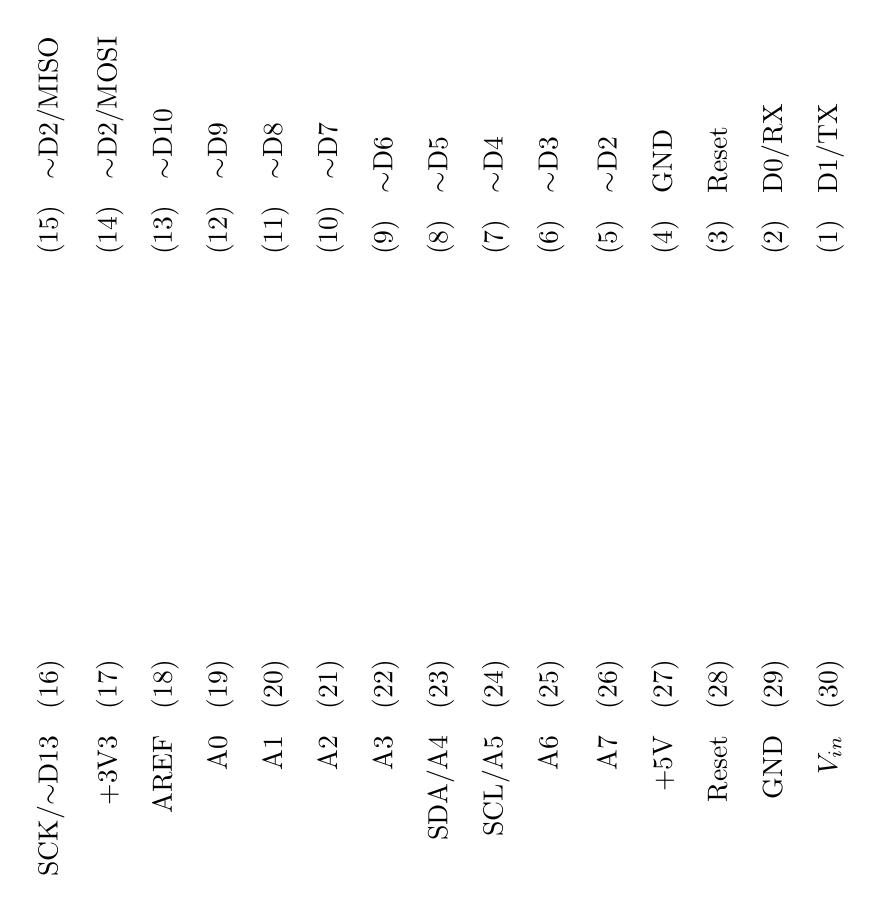
\begin{tikzpicture}
		
		\ArduinoNanoBLESenseRev
		
		\node[rotate=90,right] (Pin1) at (11.2,4.9) {(1) \; D1/TX};
		\node[rotate=90,right] (Pin2) at (10.5,4.9) {(2) \; D0/RX};
		\node[rotate=90,right] (Pin3) at (9.8,4.9) {(3) \; Reset};
		\node[rotate=90,right] (Pin4) at (9.1,4.9) {(4) \; GND};
		\node[rotate=90,right] (Pin5) at (8.4,4.9) {(5) \; $\sim$D2};
		\node[rotate=90,right] (Pin6) at (7.65,4.9) {(6) \; $\sim$D3};
		\node[rotate=90,right] (Pin7) at (6.95,4.9) {(7) \; $\sim$D4};
		\node[rotate=90,right] (Pin8) at (6.25,4.9) {(8) \; $\sim$D5};
		\node[rotate=90,right] (Pin9) at (5.55,4.9) {(9) \; $\sim$D6};
		\node[rotate=90,right] (Pin10) at (4.85,4.9) {(10) \; $\sim$D7};
		\node[rotate=90,right] (Pin11) at (4.15,4.9) {(11) \; $\sim$D8};
		\node[rotate=90,right] (Pin12) at (3.45,4.9) {(12) \; $\sim$D9};
		\node[rotate=90,right] (Pin13) at (2.75,4.9) {(13) \; $\sim$D10};
		\node[rotate=90,right] (Pin14) at (2.05,4.9) {(14) \; $\sim$D2/MOSI};
		\node[rotate=90,right] (Pin15) at (1.3,4.9) {(15) \; $\sim$D2/MISO};
		
		
		\node[rotate=90,left] (Pin30) at (11.2,-0.0) { $V_{in}$ \; (30)};
		\node[rotate=90,left] (Pin1) at (10.5,-0.0) {GND \; (29)};
		\node[rotate=90,left] (Pin2) at (9.8,-0.0) {Reset \; (28)};
		\node[rotate=90,left] (Pin3) at (9.1,-0.0) {+5V \; (27)};
		\node[rotate=90,left] (Pin4) at (8.4,-0.0) {A7 \; (26)};
		\node[rotate=90,left] (Pin5) at (7.65,-0.0) {A6 \; (25)};
		\node[rotate=90,left] (Pin6) at (6.95,-0.0) {SCL/A5 \; (24)};
		\node[rotate=90,left] (Pin7) at (6.25,-0.0) {SDA/A4 \; (23)};
		\node[rotate=90,left] (Pin8) at (5.55,-0.0) {A3 \; (22)};
		\node[rotate=90,left] (Pin9) at (4.85,-0.0) {A2 \; (21)};
		\node[rotate=90,left] (Pin10) at (4.15,-0.0) {A1 \; (20)};
		\node[rotate=90,left] (Pin11) at (3.45,-0.0) {A0 \; (19)};
		\node[rotate=90,left] (Pin12) at (2.75,-0.0) {AREF \; (18)};
		\node[rotate=90,left] (Pin13) at (2.05,-0.0) {+3V3 \; (17)};
		\node[rotate=90,left] (Pin14) at (1.3,-0.0) {SCK/$\sim$D13 \; (16)};
		
	\end{tikzpicture}
	\captionof{figure}[Pinbelegung des Arduino Nano 33 BLE Sense]{Pinbelegung des Arduino Nano 33 BLE Sense und der Rev 2 Version; Die orange Status-LED ist an Pin D13 angeschlossen, die Power-LED an Pin D1. Die RGB-LED verwendet die Pins D18, D19 und D20.}
\end{center}


\section{Pinbelegung des Arduino Nano 33 BLE}

Der Arduino Nano 33 BLE ist eine weiterentwickelte Version des Arduino Nano Boards mit dem leistungsstarken nRF52840 Prozessor. Das Board verfügt über folgende Pin-Konfiguration (siehe auch \href{https://www.etechnophiles.com/arduino-nano-33-ble-sense-pinout-introduction-specifications/}{Pin-Konfiguration}):

\begin{description}
	\item[Digitale Pins] 14 digitale I/O-Pins, die nur die Zustände HIGH oder LOW erkennen. Diese Pins können je nach Anforderung als Eingang oder Ausgang konfiguriert werden. Bei 5V liegen sie im HIGH-Zustand, bei 0V im LOW-Zustand.
	\item[Analoge Pins] 8 analoge Eingänge (A0 bis A7), die im Gegensatz zu digitalen Pins kontinuierliche Werte erfassen können. Der Messbereich liegt zwischen 0-5V.
	\item[PWM-Pins] Alle digitalen Pins können für Pulsweitenmodulation (PWM) genutzt werden, um analoge Ergebnisse mit digitalen Mitteln zu erzeugen.
	\item[SPI-Schnittstelle] Unterstützt das Serial Peripheral Interface Protokoll für die Kommunikation mit Peripheriegeräten wie Sensoren. Verwendet die Pins:
	\begin{itemize}
		\item MISO (Master Input Slave Output)
		\item MOSI (Master Output Slave Input)
	\end{itemize}
	\item[I²C-Schnittstelle] Zwei-Draht-Protokoll mit den Pins:
	\begin{itemize}
		\item SCL (Serial Clock)
		\item SDA (Serial Data)
	\end{itemize}
	\item[UART-Schnittstelle] Serielle Kommunikation über:
	\begin{itemize}
		\item Rx (Empfangs-Pin)
		\item Tx (Sendepin)
	\end{itemize}
	\item[Externe Interrupts] Alle digitalen Pins können für externe Interrupts genutzt werden, um laufende Programme bei Bedarf zu unterbrechen.
	\item[Besondere Pins]
	\begin{itemize}
		\item Pin 13: Integrierte LED
		\item AREF: Referenzspannungseingang
	\end{itemize}
\end{description}

